\chapter{評価}
\label{evaluation}
本章では,第\ref{proposal}章及び第\ref{implementation}章で設計・実装に関して述べた本提案手法に関して,第\ref{issue:siit-dc_problems}節で指摘したSIIT-DCの課題に対して有効性があることに対して定量的に評価する.



\section{評価要件}
SIIT-DCにおけるDynamicEAMT機構では,第\ref{consideration:points}節で述べた事項が求められる.
それらを定量的に評価するための指標・尺度について記述する.


\subsection{BR間のEAMTの一貫性}
第\ref{issue:siit-dc_problems:consistent}項で示したように,SIIT-DCネットワークにおける各BRは一貫性のあるEAMTを保持する必要がある.
本評価実験では後に述べるテストケースにおいて,以下の2点を検証することで各BRのEAMTが一貫性を有すると定義する.
\begin{itemize}
    \item \textbf{EAM数の収束} \\
    EAMの更新が行われる事象が発生した場合に,一定の収束時間が経過した後に各BRのEAMTのレコード数が変化することなく,一意に収束すること.
    \item \textbf{EAMTのレコードの内容} \\
    EAM数が収束した際に各BRの有するEAMTの内容に差異が無いこと.
\end{itemize}

\subsection{変更追従性}
第\ref{issue:siit-dc_problems:follow}で指摘したように,従来のSIIT-DCの構成ではIPv4サービスが追加・削除・変更された場合やBRの追加配備を行った場合に,各BRのEAMTの内容を適宜変更する必要があった.
%本評価実験では下記のN点の要素を満たすことを,EAMTがIPv4サービスの構成変更に動的に追従する状態であると定める.

本研究ではEAMT変更が必要な事象が発生した場合に,運用者が特別なオペレーションを行うことなくサービス提供を想定通りに開始・継続・中断される状況を,EAMTが変更に追従している状態であると定義する.

本評価実験では下記の様なEAMT変更が必要な事象を想定する.

\begin{itemize}
    \item \textbf{IPv4サービスの追加・削除} \\
    ネットワーク内のIPv6サービスにおいて,IPv4サービスアドレスを付与することでIPv4/IPv6の両プロトコルによるサービス提供を開始する場合.もしくは,そのサーバーが行っているIPv4サービス提供を中断する場合.
    \item \textbf{IPv4サービス提供サーバーの変更} \\
    SIIT-DCにおいて提供中のIPv4サービスに関して,他のIPv6アドレスを持つサーバーによるサービス提供を改めて開始する場合.
    \item \textbf{BRの追加・撤去} \\ 
    対外接続点に新しいBRを追加もしくは稼働中のBRを撤去しながらIPv4サービスを継続して行う場合.
\end{itemize}

% AWSのElastic LoadbalancerのTimeout時間は5秒. 1サービスアドレうあたり5秒以内に収束したら良いのでは.

\subsection{スケーラビリティ}
第\ref{consideration:points:scalability}で述べたように,DynamicEAMTを実現する機構は対外接続点やIPv4提供サービスの増加に柔軟に対応可能であることが望ましい.

本評価実験では各ノードのスケールにおいては下記を想定し,IPv4提供サービスの総数が増加した場合においても,オーダーが増加することなく動作が可能であることを評価する.

\begin{itemize}
    \item BR: 2-30ホスト 
    \item RR: 1-4ホスト 
    \item IPv4提供サーバー: 120ホスト
    \item EAM数: 0 - 10000
\end{itemize}


\section{実験環境}
本評価実験で利用した実験環境について述べる.
第\label{implementation:poc}項で記述したPoC実装を利用する.

\subsection{ネットワークトポロジー}
\begin{figure}[H]
    \begin{center}
    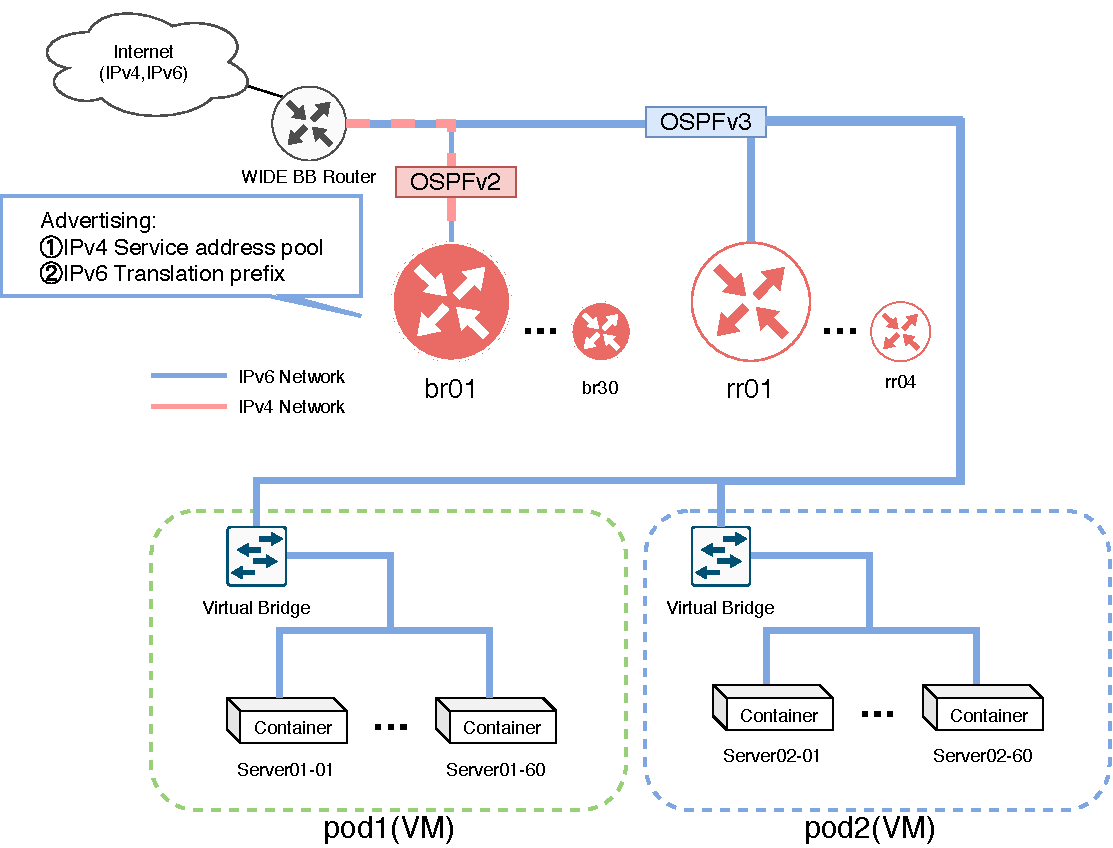
\includegraphics[width=15cm,pagebox=cropbox,clip]{img/evaluation_experiment.pdf}
    \end{center}
    \caption{評価実験におけるネットワークと各ホスト}
    \label{fig:evaluation_experiment}
\end{figure}

本評価実験を行うために,WIDEプロジェクト\footnote{\url{https://www.wide.ad.jp/}}藤沢NOC内に実験用ネットワークを構築した.図\ref{fig:evaluation_experiment}は本実験用ネットワークの概略を示す.
本ネットワークでは第\ref{issue:siit-dc-merit:scalability}項で述べたECMPエニーキャストによるBRの水平スケールを可能にするネットワークトポロジーを採用している.


本ネットワークでは,BR群(br01 $\cdots$ br30)のみWIDEネットワークを介してIPv4インターネットに接続している.WIDEプロジェクト内のルーターに対して,IPv4サービス提供サーバー群(Server01-01  $\cdots$ Server02-60)が利用するIPv4サービスアドレス群を,OSPFv2\cite{RFC2328}を利用したECMPエニーキャストにて広告する.これにより,インターネット上のIPv4クライアントからのIPv4パケットはいずれかのBRを経由し,Dynamic EAMTを参照したSIITによるネットワークプロトコル変換が各BRにて行われたのち,IPv6パケットとして各IPv4サービス提供サーバーに転送される.

各ホストは共通のIPv6ネットワーク上に所属し,WIDEプネットワークを介したインターネット疎通性を持つ.このIPv6ネットワークでは,各BRからIPv4サービス提供サーバー向けに,OSPFv3\cite{RFC5340}を利用したECMPエニーキャストによる変換プレフィックス向け経路広告が行われている.IPv4サービス提供サーバーからの変換プレフィックス宛のパケットは,いずれかのBRを経由してSIITによるネットワークプロトコル変換がなされたあと,インターネット上のIPv4提供クライアントに向けて返送される.

各ホスト間のDynamic EAMTに用いるBGPメッセージングは各ホストが共通して属するIPv6ネットワークを介して行われる.BR群及びIPv4サービス提供サーバー群はルートリフレクター群(rr01 $\cdots$ rr04)に対して,IPv6によるiBGPコネクションを確立する.本ネットワーク構成ではルートリフレクター間のBGPメッセージングは行わず,各IPv4サービス提供サーバーからの経路情報はネットワーク内で一意のクラスターIDを付与した上でBR群に広告される.

\subsection{実装}
本項では各ホストの実行環境について記述する.
各ホストが利用している,BGPデーモン・SIIT機構・SIIT制御機構の各コンポーネントは第\ref{implementation:poc:components}項で述べたPoCと同一の物を利用している.


\subsubsection{BR}
本評価ネットワークにおけるBR群は,同一物理サーバーで仮想マシンとして稼働する.
図\ref{table:eval_env_BR}に物理サーバーと仮想マシンの実行環境を詳細に示す.


\begin{table}[h]
    \label{table:eval_env_BR}
    \caption{評価実験用BR群の実行環境}
    \resizebox{\textwidth}{!}{%
    \begin{tabular}{|cccc}
    \hline
    \multicolumn{4}{|c|}{\cellcolor[HTML]{EFEFEF}\textbf{計算環境}} \\ \hline
    \multicolumn{1}{|c|}{機種} & \multicolumn{1}{c|}{CPU} & \multicolumn{1}{c|}{RAM} & \multicolumn{1}{c|}{NIC} \\ \hline
    Intel S2600WTT & 2CPU: Intel Xeon E5-2699 v3 2.30GHz & 64GB & \multicolumn{1}{c|}{Intel 82599EB 10-Gigabit SFI/SFP+} \\ \hline
    \multicolumn{4}{|c|}{\cellcolor[HTML]{EFEFEF}\textbf{ハイパーバイザー環境}} \\ \hline
    \multicolumn{1}{|c|}{OS} & \multicolumn{1}{c|}{バージョン} & \multicolumn{1}{c|}{vCPU} & \multicolumn{1}{c|}{備考} \\ \hline
    VMware ESXi & 6.7.0 & 72 & \multicolumn{1}{l|}{build: 5160138} \\ \hline
    \multicolumn{4}{|c|}{\cellcolor[HTML]{EFEFEF}\textbf{仮想マシン}} \\ \hline
    \multicolumn{1}{|c|}{OS} & \multicolumn{1}{c|}{カーネル} & \multicolumn{1}{c|}{リソース} & \multicolumn{1}{c|}{利用コンポーネント} \\ \hline
    Ubuntu 18.04.3 LTS & 4.15.0-72-generic & vCPU: 2 RAM:2GB & \multicolumn{1}{l|}{BGPデーモン,SIIT制御機構,SIIT機構} \\ \hline
    \end{tabular}%
    }
\end{table}

\subsubsection{ルートリフレクター}
本評価ネットワークにおけるBR群は,同一物理サーバーで仮想マシンとして稼働する.
図\ref{table:eval_env_RR}に物理サーバーと仮想マシンの実行環境を詳細に示す.

ルートリフレクターではGoBGPにてルートリフレクター機能に加えてダイナミックネイバー機能を有効化する.通常,BGPコネクションを確立するためにはBGPピア間で互いのピアリングアドレスを明示的に設定する必要があるが,本機能を利用することで動的に多数のBGPスピーカーとのピアリングが可能になる\cite{GoBGP_dynamic}.同様の機構は他のBGPデーモン・ネットワーク機器でも実装されている\cite{Cisco_dynamic}.


\begin{table}[]
    \label{table:eval_env_RR}
    \caption{評価実験用RR群の実行環境}
    \resizebox{\textwidth}{!}{%
    \begin{tabular}{|cccc}
    \hline
    \multicolumn{4}{|c|}{\cellcolor[HTML]{EFEFEF}\textbf{計算環境}} \\ \hline
    \multicolumn{1}{|c|}{機種} & \multicolumn{1}{c|}{CPU} & \multicolumn{1}{c|}{RAM} & \multicolumn{1}{c|}{NIC} \\ \hline
    Dell PowerEdge R410 & 2CPU: Intel Xeon E5530 @ 2.40GHz & 16GB & \multicolumn{1}{c|}{HP NC522SFP Dual Port 10GbE Server Adapter} \\ \hline
    \multicolumn{4}{|c|}{\cellcolor[HTML]{EFEFEF}\textbf{ハイパーバイザー環境}} \\ \hline
    \multicolumn{1}{|c|}{OS} & \multicolumn{1}{c|}{バージョン} & \multicolumn{1}{c|}{vCPU} & \multicolumn{1}{c|}{備考} \\ \hline
    VMware ESXi & 6.5.0 & 16 & \multicolumn{1}{l|}{build: 15256549.} \\ \hline
    \multicolumn{4}{|c|}{\cellcolor[HTML]{EFEFEF}\textbf{仮想マシン}} \\ \hline
    \multicolumn{1}{|c|}{OS} & \multicolumn{1}{c|}{カーネル} & \multicolumn{1}{c|}{リソース} & \multicolumn{1}{c|}{利用コンポーネント} \\ \hline
    Ubuntu 18.04.3 LTS & 4.15.0-72-generic & vCPU: 4 RAM:4GB & \multicolumn{1}{l|}{BGPデーモン} \\ \hline
    \end{tabular}%
    }
\end{table}

\subsubsection{IPv4サービス提供サーバー}
本実験環境において,IPv4サービス提供サーバー群はコンテナ型仮想化\cite{soltesz2007container}を利用し,二つのホスト仮想マシン上で実行される.
図\ref{table:eval_env_server}に物理サーバーとホスト仮想マシン及びコンテナの実行環境を詳細に示す.


\begin{table}[h]
    \label{table:eval_env_server}
    \caption{評価実験用IPv4サービス提供サーバー群の実行環境}
    \resizebox{\textwidth}{!}{%
    \begin{tabular}{|cccc}
    \hline
    \multicolumn{4}{|c|}{\cellcolor[HTML]{EFEFEF}\textbf{計算環境}} \\ \hline
    \multicolumn{1}{|c|}{機種} & \multicolumn{1}{c|}{CPU} & \multicolumn{1}{c|}{RAM} & \multicolumn{1}{c|}{NIC} \\ \hline
    Dell PowerEdge R410 & 2CPU: Intel Xeon E5530 @ 2.40GHz & 48GB & \multicolumn{1}{c|}{HP NC522SFP Dual Port 10GbE Server Adapter} \\
    \multicolumn{1}{|l}{Dell PowerEdge R410} & \multicolumn{1}{l}{2CPU: Intel Xeon E5530 @ 2.40GHz} & 48GB & \multicolumn{1}{l|}{HP NC522SFP Dual Port 10GbE Server Adapter} \\ \hline
    \multicolumn{4}{|c|}{\cellcolor[HTML]{EFEFEF}\textbf{ハイパーバイザー環境}} \\ \hline
    \multicolumn{1}{|c|}{OS} & \multicolumn{1}{c|}{バージョン} & \multicolumn{1}{c|}{vCPU} & \multicolumn{1}{c|}{備考} \\ \hline
    VMware ESXi & 6.5.0 & 16 & \multicolumn{1}{l|}{build: 15256549. Pod1,Pod2で共通} \\ \hline
    \multicolumn{4}{|c|}{\cellcolor[HTML]{EFEFEF}\textbf{ホスト仮想マシン}} \\ \hline
    \multicolumn{1}{|c|}{OS} & \multicolumn{1}{c|}{カーネル} & \multicolumn{1}{c|}{リソース} & \multicolumn{1}{c|}{備考} \\ \hline
    Ubuntu 18.04.3 LTS & 4.15.0-72-generic & vCPU: 4 RAM:4GB & \multicolumn{1}{l|}{Pod1, Pod2で共通} \\ \hline
    \multicolumn{4}{|c|}{\cellcolor[HTML]{EFEFEF}\textbf{コンテナ}} \\ \hline
    \multicolumn{1}{|c|}{OS} & \multicolumn{1}{c|}{コンテナエンジン} & \multicolumn{1}{c|}{コンテナイメージ} & \multicolumn{1}{c|}{利用コンポーネント} \\ \hline
    Alpine Linux 3.11 & Dockerversion 19.03.5 & 自作 & \multicolumn{1}{l|}{GoBGPデーモン} \\ \hline
    \end{tabular}%
    }
\end{table}

\subsubsection{経路注入用サーバー}
本提案手法のスケーラビリティをより効率的に検証するために,各ルートリフレクターに任意の数の経路を広告するサーバー(Injector)を設置する.
実行環境はIPv4サービス提供サーバーと同一であるが,IPv4サービス提供サーバーは自身のIPv4サービスアドレスを一つ広告するのに対して,本サーバーは実際にはサービス提供に利用できないダミー経路を広告する.


\section{実験シナリオ1: SIIT-DCネットワークの構築}
このシナリオにおける,BRの数, サーバーの数を変数とした時に変化を調べる.

\subsection{ネットワーク構成}
図を張る. BRとサーバーは水平スケールさせる.


\subsection{実験結果}
EAMTが一貫するまでの時間を調べる.

\subsection{考察}
一貫性保持が成功.

線形に変化しており,O(n)の十分なスケーラビリティがある.


\section{実験シナリオ2: サーバーの構成変更}
このシナリオにおける,BRの数, サーバーの数を変数とした時に変化を調べる.

サーバーの削除からのFailover(LPで重み替え)



\subsection{ネットワーク構成}
図を張る. BRとサーバーは水平スケールさせる.

\subsection{実験結果}
追加したサーバー1台がサービス開始出来るまでの時間を,サーバー台数とBR台数が増えていった場合にも変わらず出来ることを証明.


\subsection{考察}
リニアに追従.

線形に変化しており,O(n)の十分なスケーラビリティがある.


%%% Local Variables:
%%% mode: japanese-latex
%%% TeX-master: "../thesis"
%%% End:
